\chapter{La communication vibratoire}

De nombreux animaux communiquent par l'intermédiaire de vibrations : les
punaises vertes (\emph{Nezara virudula}) communiquent à l'aide de
vibrations transmises par les feuilles sur lesquelles elles se trouvent
lors de leur parade amoureuse. De même, les éléphants émettent des
signaux vibratoires en frappant le sol de leurs pattes pouvant être
reçus par d'autres éléphants à plusieurs kilomètres de distances, selon
\href{http://www.ncbi.nlm.nih.gov/pubmed/11144599}{une étude de
\textsc{O'Connell-Rodwell}}. Par ailleurs, les araignées communiquent
par des vibrations transmises dans la toile et celle ci présente de
nombreux aspects : elle est utilisée non seulement lors de la parade
amoureuse, mais aussi au sein de sociétés d'araignées sociales et permet
la détection d'intrus ou de proie. De plus, le substrat, c'est-à-dire la
base matérielle, le support de la communication vibratoire chez les
araignées est tout à fait particulier : ce sont les fils de soie,
produits par les araignées.

Les araignées ont à leur disposition différents types de signaux pour
communiquer. Tout d'abord, des signaux visuels, notamment lors de la
parade amoureuse même si elles ont une très mauvaises vue, mais aussi
des signaux sonores, en effet les araignées stridulent en frottant
différentes parties de leur corps, des signaux chimiques, en effet comme
toutes les espèces animales, les araignées communiquent par
l'intermédiaire de phéromones, mais c'est bien la communication
vibratoire qui est prédominante chez les araignées.

Toutefois, l'étude de la communication vibratoire est très récente,
c'est Peter N.~\textsc{Witt}, en 1982 qui le premier l'étudia en
profondeur dans son ouvrage \emph{Spider Communication} (TODO : mettre
numéro livre), dans lequel il s'intéresse à la communication entre
araignées et à la détection des proies, suivant la définition large de
la communication comme tout comportement qui transmet une information
d'un individu à un autre.

(TODO: interesserons à araignée + annonce plan)

\section{Rôle de la communication vibratoire chez les araignées}

La communication vibratoire permet principalement aux araignées de
repérer des proies et des partenaires sexuels. On peut ensuite définir
deux types d'araignées : les araignées sociales et les araignées
solitaires. Les araignées solitaires n'ont recours à la communication
avec d'autres araignées que lorsqu'elles rencontrent une toile, alors
que pour les espèces sociales, soit environ douze genres d'araignées,
c'est-à-dire douze regroupements d'espèces, la communication vibratoire
a un rôle majeur : elle leur permet d'organiser leur vie en société, et
elle leur permet notamment d'organiser la capture des proies en groupe.

De plus, toutes les espèces sociales sont fileuses, elles organisent
leur vie dans des structures soyeuses atteignant souvent un volume de
100m3 (voir~Figure~1). Ces structures soyeuses, qu'elles ne quittent
jamais, favorisent la communication vibratoire. Tout comme pour les
araignées solitaires, les vibrations dans la toile leur permettent
d'être alertées de la présence d'intrus et de proies : dès qu'un insecte
est pris au piège dans la toile, une horde d'araignées l'encercle, le
tue puis s'en nourrit. Dès lors, on peut en déduire que la communication
vibratoire permet à l'araignée de distinguer ses congénères des proies,
et lui permet aussi de localiser la proie sur la toile.

\begin{figure}[htb!]
	\centering
	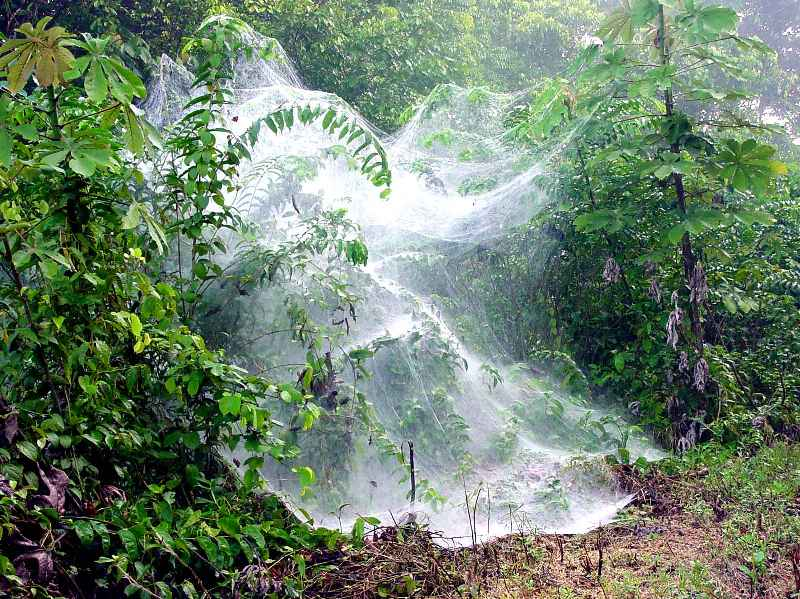
\includegraphics[width=0.7\linewidth]{../img/vibrations/toileSociale}
	\caption{Toile d'une société d'Anolesimius Eximius, espèce
		d'araignée sociale (photographie de B. \textsc{Krafft}}
	\label{fig:toileSociale}
\end{figure}


Les araignées utilisent aussi les vibrations dans la toile d'une manière
qui rappelle l'écholocation chez les chauves-souris ou les dauphins :
lorsqu'une proie se tient immobile sur la toile, l'araignée peut envoyer
une secousse dans la toile qui provoquera le balancement de la proie, et
permettra sa localisation.

Mais certaines araignées utilisent aussi à leur profit la capacité
d'autres insectes à communiquer. Par exemple, les sauterelles
communiquent normalement par sons qui se propagent dans l'air, mais
elles peuvent aussi communiquer par vibrations dans les plantes pour
éviter d'attirer les chauves-souris, ces vibrations sont utilisées par
les araignées pour localiser les sauterelles, et les chasser. De même,
l'araignée sauteuse commune, \emph{Portia fimbriata}, est capable
d'imiter les signaux vibratoires de mâles d'autres espèces d'araignée
afin d'attirer les femelles, qu'elle chasse.

\section{Production des signaux vibratoires}

Les araignées ont recours à différentes méthodes pour produire des
vibrations dans un substrat : les percussions, les vibrations du corps,
les stridulations et en tirant directement sur la toile.

\subsection{La percussion}

En frappant le sol de son abdomen ou de son pédipalpe (voir Figure 2),
l'araignée peut créer des vibrations qui se propagent dans le sol. La
force du signal vibratoire est directement lié à la masse de l'animal à
l'origine de la vibration, plus l'animal est massif et plus le rayon de
propagation est large.


\begin{figure}[htb!]
	\centering
	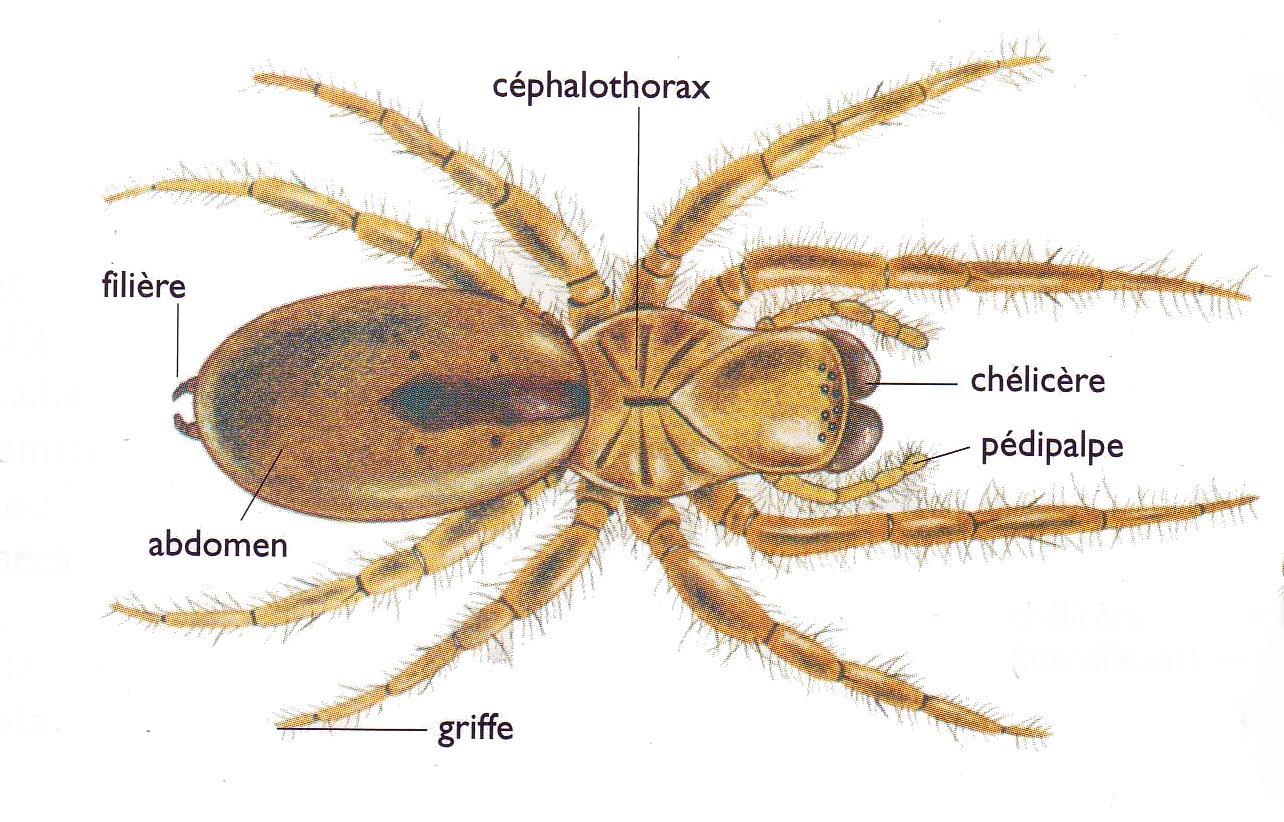
\includegraphics[width=0.7\linewidth]{../img/vibrations/anatomie_araignee}
	\caption{Anatomie d'une araignée}
	\label{fig:anatomie_araignee}
\end{figure}


Ce type d'émission est utilisé surtout par les espèces qui ne font pas
de toile, comme les araignées sauteuses (\emph{Salticidae}) ou les
araignées-loups (\emph{Lycosidae}). Ainsi, le mâle \emph{Lycosa gulosa}
produit des sons qui pourront être perçus par la femelle en frappant le
sol de ses pédipalpes.

\subsection{La trémulation}

Les araignées peuvent faire vibrer leur corps afin d'émettre des
vibrations qui passeront à travers leurs pattes puis dans le sol, c'est
ce qu'on appelle la trémulation. La trémulation ne nécessite pas une
morphologie particulière, mais la fréquence des vibrations produites est
souvent très faible, car elle est limitée par la vitesse à laquelle
l'animal peut faire vibrer son corps, dès lors, elle est donc
difficilement analysable.

\subsection{La stridulation}

Les araignées, comme certains insectes, peuvent striduler, c'est-à-dire
produire des vibrations en frottant deux parties de leur corps. Ces
vibrations sont ensuite transmises au sol par les pattes, et dans l'air
sous la forme de sons audibles. Une araignée peut striduler en frottant
son abdomen et son céphalothorax, ou en frottant différents appendices,
comme patte contre patte, patte contre pédipalpe ou chélicère contre
chélicère (voir Figure 2).

\subsection{Le tiraillement}\label{le-tiraillement}

Les araignées peuvent aussi tirer sur les fils de la toile à l'aide de
leur pattes pour y transmettre des vibrations, par exemple en exerçant
une forte traction sur la toile puis en relâchant rapidement cette
tension, envoyant un signal de grande amplitude.

\begin{figure}[htb!]
	\centering
	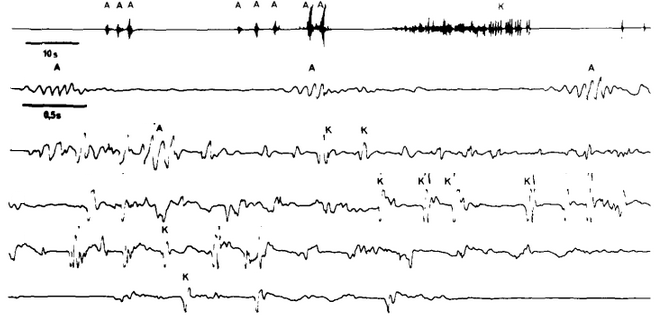
\includegraphics[width=0.7\linewidth]{../img/vibrations/SignalSpiders}
	\caption{Vibrations émises par un mâle Tegenaria parietina
		dans la toile. A : trémulations abdominales ; K : percussions avec
		l'abdomen (d'après \textsc{Leborgne} et \textsc{Krafft}, 1979)}
	\label{fig:SignalSpiders}
\end{figure}

Afin que les signaux soient reconnaissables, les araignées produisent
des vibrations caractéristiques en faisant varier la fréquence et
l'amplitude des vibrations, ainsi que la répartition de ces vibrations
au cours du temps. Nous pouvons voir cette variation du motif des
vibrations en Figure 3, on peut remarquer la répétition des trois
trémulations abdominales.

\section{Transmission du signal vibratoire}

Une fois produit par l'araignée, la vibration se propage dans le
substrat, la plupart du temps de la soie d'araignée. C'est pourquoi nous
avons effectué différentes expériences pour étudier les propriétés de la
soie d'araignée.

\subsection{Analyse microscopique}

Nous avons procédé à une analyse microscopique de fil de soie
d'araignée. Afin d'avoir les fils, nous avons capturé une araignée qui a
ensuite fait sa toile dans une boite. Grâce à un appareil photo
numérique pour microscope, nous avons pu obtenir des clichés du fil
d'araignée.

	\begin{figure}[htb!]
		\centering
		\begin{subfigure}{.5\textwidth}
			\centering
			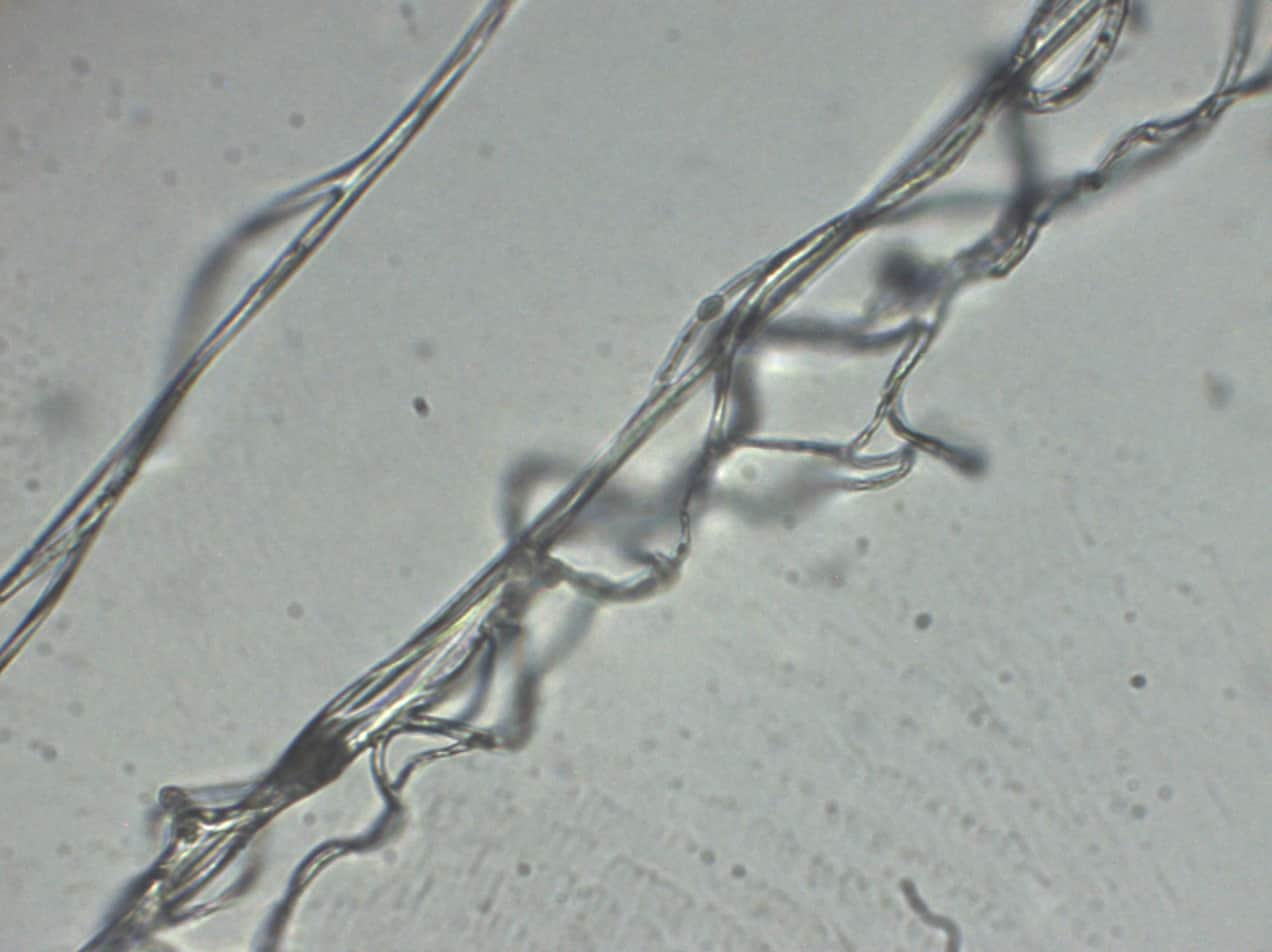
\includegraphics[width=0.8\linewidth]{../img/vibrations/FilMicroscopeA}
			\caption{}
			\label{fig:FilMicroscopeA}
		\end{subfigure}%
		\begin{subfigure}{.5\textwidth}
			\centering
			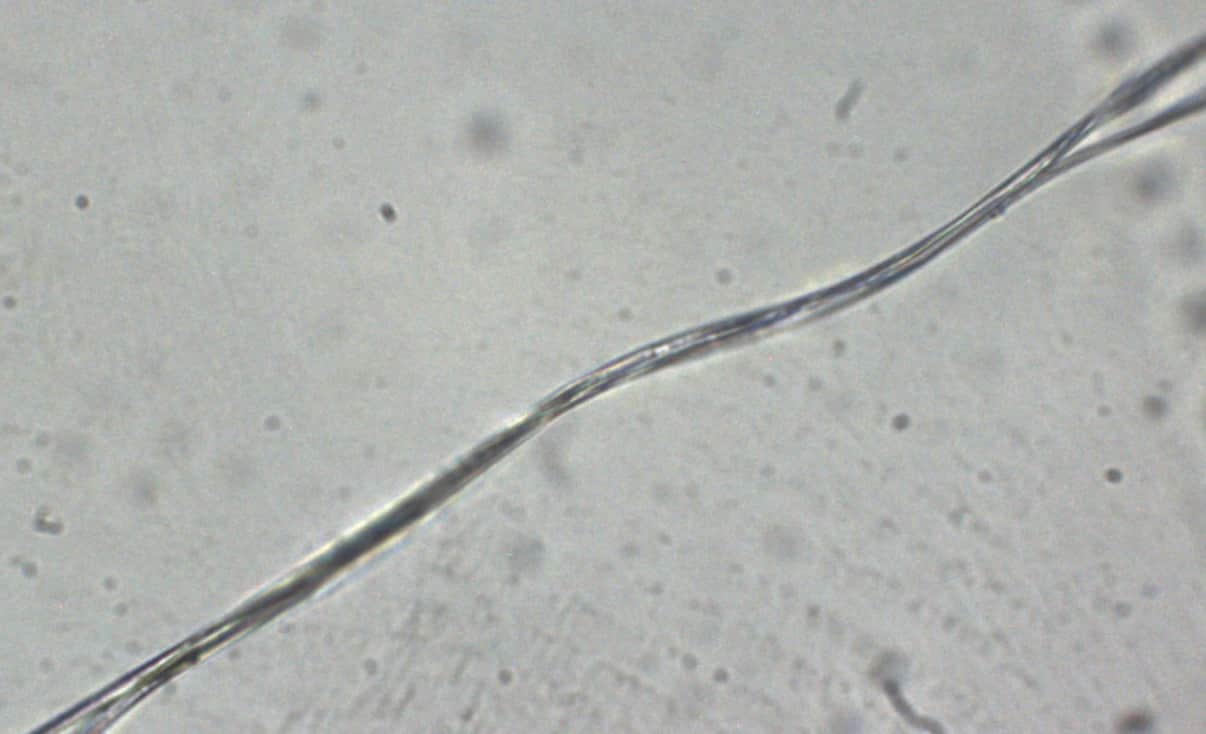
\includegraphics[width=0.8\linewidth]{../img/vibrations/FilMicroscopeB}
			\caption{}
			\label{fig:FilMicroscopeB}
		\end{subfigure}
		\caption{Photographies de fils d'araignée vus au microscope optique (×600)}
		\label{fig:test}
	\end{figure}

Le premier fil n'a pas été coloré, et le second a été coloré au bleu de
méthylène. Nous pouvons voir sur ces photographies que les fils
d'araignée sont en fait constitués de plusieurs fils tressés les uns
autour des autres, toutefois la coloration au bleu de méthylène ne
permet pas de différencier différente partie dans chacun des fils.

\subsection{Mesure de la taille d'un fil de soie d'araignée}

Afin d'étudier plus précisément le fil d'araignée, nous avons souhaité
mesurer son diamètre. Ceci est possible en analysant le phénomène de
diffraction ayant lieu lorsqu'un laser rencontre ce fil d'araignée,
c'est-à-dire la manière dont la lumière est diffusée après avoir
rencontré le fil.

Lorsqu'on projette la lumière après le fil sur un écran, on obtient des
tâches, et la taille de la tâche centrale (mesurée à partir des milieux
entre la tâche centrale et les tâches autour de la tâche centrale) est
inversement proportionnelle au diamètre du fil.

C'est pourquoi à l'aide d'un montage composé d'une diode laser, d'un
écran et d'un fil dans une diapositive positionnée entre la diode et
l'écran, à un mètre de l'écran, on peut former les tâches sur l'écran et
mesurer la taille de la tâche centrale, comme vu en Figure 5.

\begin{figure}[htb!]
	\centering
	\def\svgwidth{\columnwidth}
	\input{../img/vibrations/schemaDiffraction.pdf_tex}
	\caption{Montage pour mesurer la taille du fil de soie}
\end{figure}

Afin de pouvoir calculer le coefficient de proportionnalité entre le
diamètre du fil et l'inverse de la largeur de la tâche centrale, on
mesure la taille de la tâche centrale pour des fils de diamètre connu.
Par ailleurs on mesure la taille de la tâche centrale d'une lumière de
laser diffracté par un fil d'araignée \emph{A}, puis d'un fil \emph{B},
prélevé sur la toile de l'araignée capturée. Avec ces mesures, on
obtient le tableau suivant.

\begin{tabu}[c]{@{}rrr@{}}
	\toprule
	Diamètre fil (mm) & Largeur L de la tâche centrale (mm) & 1 /
	L\tabularnewline
	\midrule
	
	D(filA) & 1,08×102 & 9,26×10-3\tabularnewline
	D(filB) & 8,0×101 & 1,25×10-2\tabularnewline
	4,0×10-2 & 3,3×101 & 3,0×10-2\tabularnewline
	6,0×10-2 & 2,2×101 & 4,6×10-2\tabularnewline
	1,0×10-1 & 1,3×101 & 7,7×10-2\tabularnewline
	1,2×10-1 & 1,1×101 & 9,1×10-2\tabularnewline
	\bottomrule
\end{tabu}

Ces mesures permettent de tracer un graphique. La proportionnalité entre
le diamètre du fil et la taille de la tâche centrale est modélisée par
une droite de coefficient directeur 0,76 et passant par l'origine du
repère.

\begin{figure}[htb!]
	\centering
	\def\svgwidth{\columnwidth}
	\input{../img/vibrations/graphiqueDiffraction.pdf_tex}
	\caption{\(1 / L\) en fonction du diamètre du fil}
\end{figure}

Dès lors on peut calculer :

\( D(fil) = \frac{\frac{1}{L}}{0.76}\)

Donc: 
\(D(filA) = \frac{9,26\times10^{-3}}{0.76}\)


\(D(filA) = 1,2\times10^{-2} \text{mm} = 1,2\times10^{-5} \text{m} = 12 \mu\text{m}\)

Et,

\(D(filB) = \frac{1,25\times10^{-2}}{0.76}\)


\(D(filB) = 1,6\times10^{-2} \text{mm} = 1,6\times10^{-5} \text{m} = 16 \mu\text{m}\)

Ainsi, selon nos mesures un fil de soie d'araignée a une taille moyenne
de \( \bar{x} = \frac{D(filA) + D(filB)}{2} = \frac{12 + 16}{2} = 14 \mu\text{m}\), soit environ un dixième de la taille d'un cheveu.

Ainsi, même si le fil de soie d'araignée est extrêmement fin, les
araignées sont capables de construire des toiles résistantes au poids de
l'araignée elle-même, à celui d'éventuels intrus et à la transmission
d'ondes, notamment dans le cadre de la communication.

\subsection{Vitesse d'une onde dans la toile}

Les vibrations émises par l'araignée prennent la forme d'ondes
mécaniques progressives dans la toile, c'est-à-dire la propagation d'une
perturbation dans un milieu matériel sans transport de matière. Cette
onde est dite à une dimension puisqu'elle ne se propage que dans une
seule direction.

Afin d'étudier la vitesse d'une onde dans la toile, nous avons décidé de
nous intéresser à la vitesse d'une onde dans une corde. Pour cela nous
avons mesuré le temps que prenait une onde pour parcourir un mètre sur
deux cordes, corde A et corde B à l'aide de deux capteurs laser, en
tendant plus ou moins la corde, comme vu en Figure 7.

\begin{figure}[htb!]
	\centering
	\def\svgwidth{\columnwidth}
	\input{../img/vibrations/schemaVOnde.pdf_tex}
	\caption{Montage pour mesurer la vitesse de propagation d'une onde dans une corde}
\end{figure}

Corde A :

Masse de la corde : \(m_A = 4,6\times10^{-2} \text{kg}\)

Longueur de la corde : \(L_A = 2,08 \text{m}\)

Masse linéique (masse par unité de longueur) :

\(\mu_A = \frac{m}{L} = \frac{4,6\times10^{-2}}{2,08} = 2,2\times10^{-2} \text{kg.m}^{-1}\)
\begin{table}
	\centering
	\begin{tabu}[c]{@{}llllll@{}}
		\toprule
		Tension & A & B & C & D \tabularnewline
		\midrule
		& 24 & 19 & 10 & 5 \tabularnewline
		
		& 22 & 18 & 13 & 4 & \  \tabularnewline
		& 26 & 15 & 6 & 7 & \  \tabularnewline
		& 26 & 15 & 9 & 4 & \  \tabularnewline
		& 20 & 15 & 11 & 9 & \  \tabularnewline
		& 28 & 22 & 7 & 6 & \  \tabularnewline
		& 23 & 15 & 9 & 6 & \  \tabularnewline
		& 17 & 14 & 10 & \  & \  \tabularnewline
		& 8 & \  & \  & \  & \  \tabularnewline
		& 5 & \  & \  & \  & \  \tabularnewline
		\midrule
		Moyenne & 24 & 17 & 9.2 & 6 \tabularnewline
		\bottomrule
		
		
	\end{tabu}
	\caption {Durée Δt (s) que prend la vibration à parcourir un mètre sur la corde A en fonction de la tension (avec A<B<C<D)}
\end{table}



Corde B :

Masse de la corde : \(m_B = 2,1\times10^{-1} \text{kg}\)

Longueur de la corde : \(L_B = 3,07 \text{m}\)

Masse linéique (masse par unité de longueur) :
\(\mu_B = \frac{2,1\times10^{-1}}{3,07} = 7,0\times10^{-2} \text{kg.m}^{-1} > \mu_A\)
\begin{table}
	\centering
	\begin{tabu}[c]{@{}llll@{}}
		\toprule
		Tension & A' & B' &  \tabularnewline
		\midrule
		& 30 & 28 & \  \tabularnewline
		& 35 & 31 & \  \tabularnewline
		& 39 & 35 & \  \tabularnewline
		& 30 & 23 & \  \tabularnewline
		& 35 & 17 & \  \tabularnewline
		& 41 & 35 & \  \tabularnewline
		& 36 & 27 & \  \tabularnewline
		& 45 & 33 & \  \tabularnewline
		& 37 & 37 & \  \tabularnewline
		& 37 & 37 & \  \tabularnewline
		\midrule
		Moyenne & 36.5 & 30.3 & \  \tabularnewline
		\bottomrule
	\end{tabu}
	\caption {Durée Δt (s) que prend la vibration à parcourir un mètre sur la corde B en fonction de la tension (avec A'<B')}
\end{table}




Dès lors on peut remarquer que plus la tension de la corde est élevée,
et plus la propagation se déplace rapidement dans la corde, et plus la
corde a une masse linéique élevé, et plus la propagation se déplace
lentement.

Le calcul théorique de la vitesse \(v\) d'une onde dans une corde est
\(v = \sqrt{\frac{T}{\mu}}\), où \(T\) est la tension de la corde et
\(\mu\) sa masse linéique, ce qui est en accord avec nos observations.

Selon
\href{http://web.mit.edu/course/3/3.064/www/slides/Ko_spider_silk.pdf}{une
étude menée conjointement par des universités américaines et
japonaises}, la masse linéique d'une fibre de soie d'araignée est
\(\mu_{fibre} = 1,4\times10^{-8} \text{kg.m}\)-1, même s'il est composé
de plusieurs fibres, le fil de soie d'araignée a une masse linéique
extrêment faible. Par ailleurs, la toile est sous tension. Les ondes se
déplacent donc extrêmement rapidement dans la toile, ce qui est un des
atouts majeurs de la communication vibratoire pour les araignées.

\section{Perception des signaux vibratoires}

Les araignées perçoivent très bien les signaux vibratoires, en effet,
elles sont dotées de différents organes leur permettant de recevoir des
vibrations, notamment les trichobotries et les sensilles en fente, ce
sont les organes mécanorécepteurs.

\subsection{Les trichobotries}

Les trichobotries sont des soies sensorielles fines, longues et
extrêmement mobiles insérées dans une cupule (une petite structure de la
forme d'une coupe), et reliées à un nerf par un dendrite, une courte
extension des cellules nerveuses (voir Figure 8).

\begin{figure}[htb!]
	\centering
	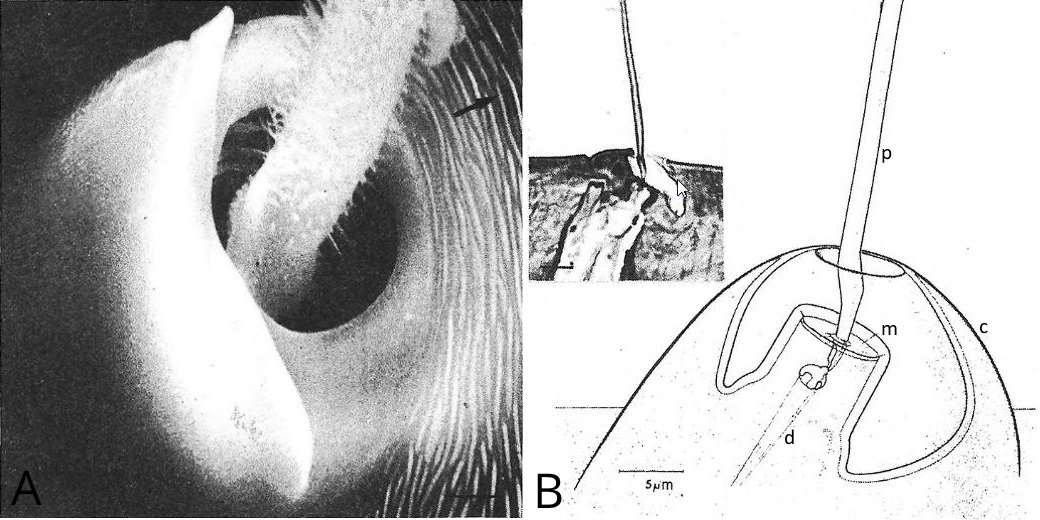
\includegraphics[width=0.7\linewidth]{../img/vibrations/trichobotrie}
	\caption{A : Base d'une trichobotrie, montrant la cupule et
		la structure plumeuse du poil ; B : Structure d'une trichobotrie (p :
		poil, c : cupule, m : membrane, d : dentrite)}
	\label{fig:trichobotrie}
\end{figure}


Les trichobotries sont disposées sur les pattes et les pédipalpes de
l'araignée. Ayant une masse très faible, étant extrêmement flexible et
étant en contact avec l'air autour de l'araignée, les trichobotries
permettent la détection de mouvement dans l'air, mais aussi dans le
substrat.

\subsection{Les sensilles en fente}

Les sensilles en fente sont des petits organes mécanorécepteurs qui
peuvent détecter la déformation ou la tension. Elles se situent sur
l'intégralité de l'exosquelette (aussi appelé cuticule) de l'araignée,
et notamment sur les pattes. Leur apparence de fente est à l'origine de
leur nom, mais elles ne pénètrent en fait pas l'exosquelette, elles
correspondent à un amincissement de la cuticule.

Elles prennent la forme de petites fentes de 1 à 2µm de large et entre 8
et 200µm de long, et peuvent être situées seules ou en groupe (voir
Figure 9). Un groupe de sensilles en fente est appelé un organe
lyriforme, car, les fentes étant parallèles entre elles, il a la forme
d'une lyre, et une sensille en fente seule est appelé sensille en fente
simple.

\begin{figure}[htb!]
	\centering
	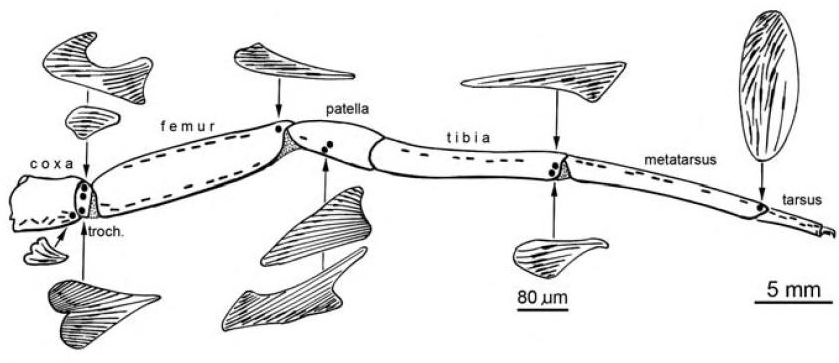
\includegraphics[width=0.7\linewidth]{../img/vibrations/Sensilles}
	\caption{Distribution des sensilles en fente sur l'arrière
		de la première patte d'une Cupiennus salei : les traits indiquent des
		sensilles en fente seule, et les points des organes lyriformes (enlargis
		pour voir les détails) (d'après \textsc{Barth} et \textsc{Libera},
		1870)}
	\label{fig:Sensilles}
\end{figure}

La fente est bordée d'une lèvre cuticulaire et est recouverte d'une
membrane cuticulaire. Sous la membrane, une sorte de gouttière s'étend
vers le bas et s'élargit en prenant la forme d'une cloche, où se
trouvent deux dendrites qui relient la sensille en fente au nerf (voir
Figure 10). Même une tension très faible au niveau de la cuticule
causera une déformation de la sensille, et la membrane se pliera,
déformant l'extrémité d'une des dendrites, provoquant un signal nerveux.

\begin{figure}[htb!]
	\centering
	\def\svgwidth{\columnwidth}
	\input{../img/vibrations/Sensilles2.pdf_tex}
	\caption{Schéma d'une sensille simple d'une Cupiennius (d'après \textsc{Barth}, 1971}
\end{figure}

C'est en analysant la différence de temps entre l'arrivée de la
vibration dans ses différentes pattes que l'araignée peut déterminer la
direction de la proie ou de l'intrus.

\section{Utilisation des connaissances en matière de communication vibratoire}

\subsection{Dans la lutte intégrée}

Les connaissances en matière de communication vibratoire peuvent être
utilisé de différentes manière. En effet, en étant capable de reproduire
ou d'imiter des signaux vibratoires, il est possible d'agir sur le
comportement des animaux ayant recours à ce type de communication. Ceci
est intéressant notamment dans le cadre de la lutte intégrée, définie en
Europe par la directive communautaire 91/414/CEE du 15 juillet 1991
ainsi :

\begin{quote}
« L'application rationnelle d'une combinaison de mesures biologiques,
biotechnologiques, chimiques, physiques, culturales ou intéressant la
sélection des végétaux dans laquelle l'emploi de produits chimiques
phytopharmaceutiques est limité au strict nécessaire pour maintenir la
présence des organismes nuisibles en dessous de seuil à partir duquel
apparaissent des dommages ou une perte économiquement inacceptables. »
\end{quote}

Ainsi, il serait possible de contrôler sans utiliser de pesticides des
populations d'insectes nuisibles ayant recours à la communication
vibratoire, comme la cicadelle de la vigne (\emph{Scaphoideus titanus}).
Les cicadelles n'utilisent pas de communication chimique à longue
portée, mais peuvent transmettre des signaux vibratoires à travers les
feuilles de vigne jusqu'à plusieurs mètres de distances. Or, la
cicadelle de la vigne est officiellement reconnue comme \emph{nuisible}
car elle est responsable de la propagation de la flavescence dorée,
maladie à l'origine de pertes importantes de récoltes de vignes, et son
contrôle est donc obligatoire.

Dans son article
\href{http://journals.plos.org/plosone/article?id=10.1371/journal.pone.0032954}{«
Exploitation of Insect Vibrational Signals Reveals a New Method of Pest
Management »}, Anna \textsc{Eriksson} (et al.) étudie l'utilisation de
vibrations pour perturber la communication entre mâles et femelles
\emph{Scaphoideus titanus} en envoyant des signaux pré-enregistrés que
les mâles \emph{Scaphoideus titanus} utilisent pour empêcher les autres
mêles de s'accoupler.

\begin{figure}[htb!]
	\centering
	\def\svgwidth{\columnwidth}
	\input{../img/vibrations/graphiqueLutteIntegree.pdf_tex}
	\caption{Nombre de femelles non fécondées trouvées sur les feuilles de vigne (A) sur des plantes en pot, (B) dans un champ de vigne, selon la distance de la source de vibrations.},
\end{figure}

Après avoir effectué et analysé des essais, elle a obtenu des résultats
concluants que cette méthode de contrôle est très efficace (voir Figure
11) : même lorsque la source de vibration se trouve à 940cm, plus de 80
\% des femelles restent non fécondées, alors que dans le cas du groupe
contrôle (non montré sur le graphique) seuls 20 \% des femelles
restaient non fécondées.

Cette méthode agit donc fortement sur la population, car non seulement
elle empêche la fécondation d'une grande partie des femelles, mais elle
retarde de plus les fécondations ayant lieu, la femelle est donc moins
féconde qu'elle ne l'aurait été. Ainsi, l'utilisation de signaux
vibratoires pour perturber la reproduction s'accorde bien à la
définition de la lutte intégrée, car en empêchant, ou du moins en
retardant la fécondation, elle permet de diminuer la population de
nuisible sans l'exterminer, tout en limitant l'utilisation de produits
chimiques.

Toutefois, dans
\href{http://onlinelibrary.wiley.com/enhanced/doi/10.1002/ps.3848}{une
étude plus récente} Jernej \textsc{Polajnar}, Anna \textsc{Eriksson} et
al. ont mis en évidences l'existence d'effets secondaires causés par la
production de signaux vibratoires, notamment la perturbation d'insectes
non nuisibles comme les abeilles ou les araignées.

De plus, ils soulignent les limitations techniques de cette méthode :
l'atténuation des vibrations est extrêmement rapide dans la plupart des
milieux solides. Toutefois certains insectes ont surmonté cette
difficulté en produisant des vibrations proches de fréquences
résonnantes du substrat, c'est-à-dire les fréquences auxquelles le
substrat est sensible, et qui, répétés sous forme périodique, provoquera
l'accumulation d'énergie dans le substrat jusqu'à atteindre un régime
d'équilibre. Il est donc possible d'imiter les fréquences utilisées par
les insectes pour diminuer l'importance du problème d'atténuation.

Par ailleurs, la situation du champ de vignes étudiés par Anna
\textsc{Eriksson} était une situation idéale, car les vignes forment une
ligne et chaque pied de vigne est relié au suivant, facilitant la
transmission de vibrations d'un pied de vigne au suivant. Dès lors, on
peut se demander si cette méthode est vraiment applicable


\subsection{Bibliographie}
